\mode*

\section{Distance bounding}

\subsection{Some scenarios}

\begin{frame}
  \begin{figure}
    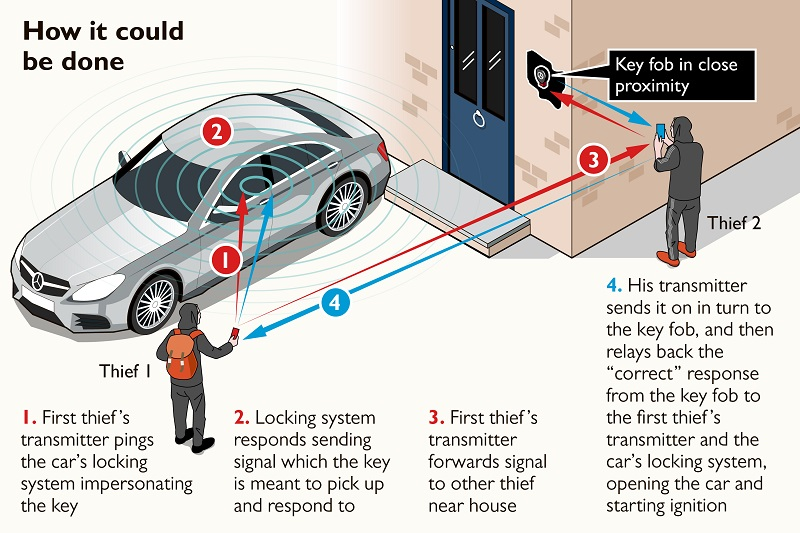
\includegraphics[width=0.8\columnwidth]{keyless-car-theft.jpg}
    \caption{%
      How does the car know the key is close to the car?
      Image: Business Motoring.
    }
  \end{figure}
\end{frame}

\begin{frame}
  \begin{figure}
    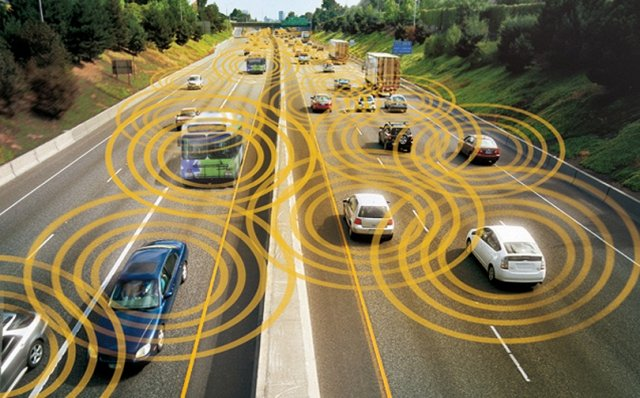
\includegraphics[width=0.8\columnwidth]{v2v-communication.jpg}
    \caption{%
      How can a car know that the other car is \emph{actually} there?
      Image: NHTSA.
    }
  \end{figure}
\end{frame}

\begin{frame}
  \begin{figure}
    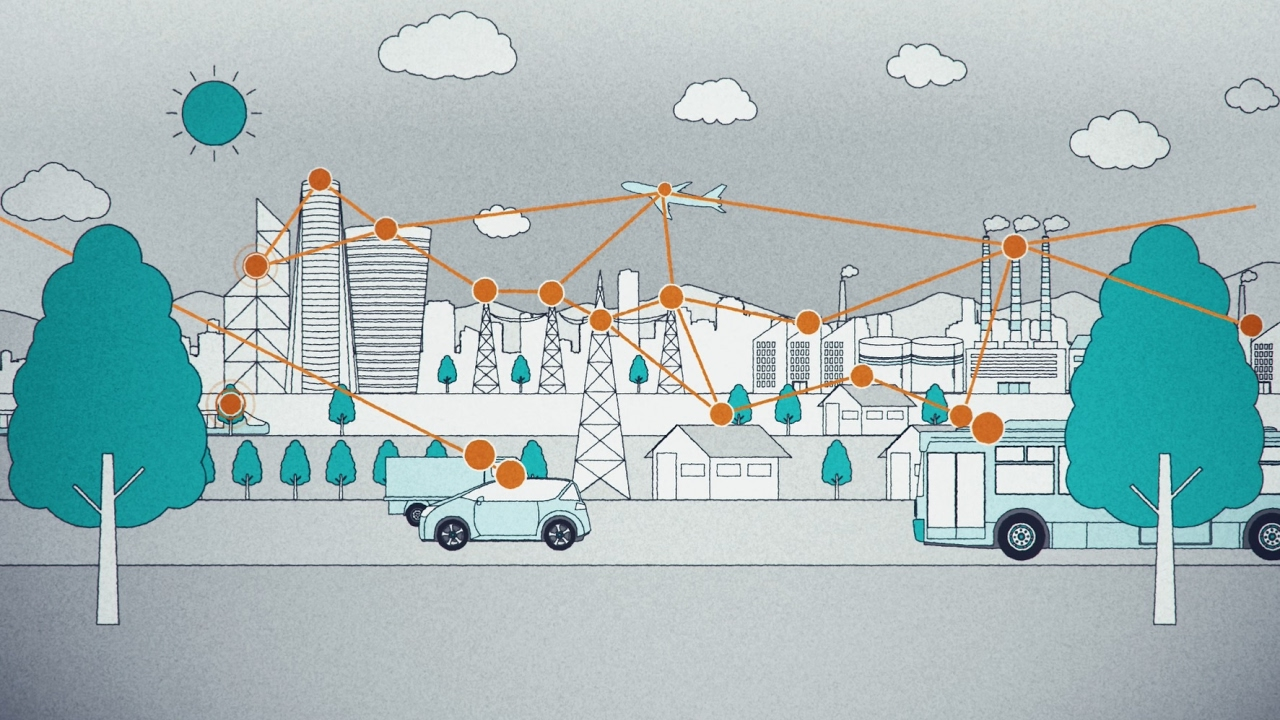
\includegraphics[width=0.8\columnwidth]{sensor-networks.jpg}
    \caption{%
      How does a sensor in a sensor network know the other sensors are where 
      they claim?
      Image: Toshiba.
    }
  \end{figure}
\end{frame}

\begin{frame}
  \begin{figure}
    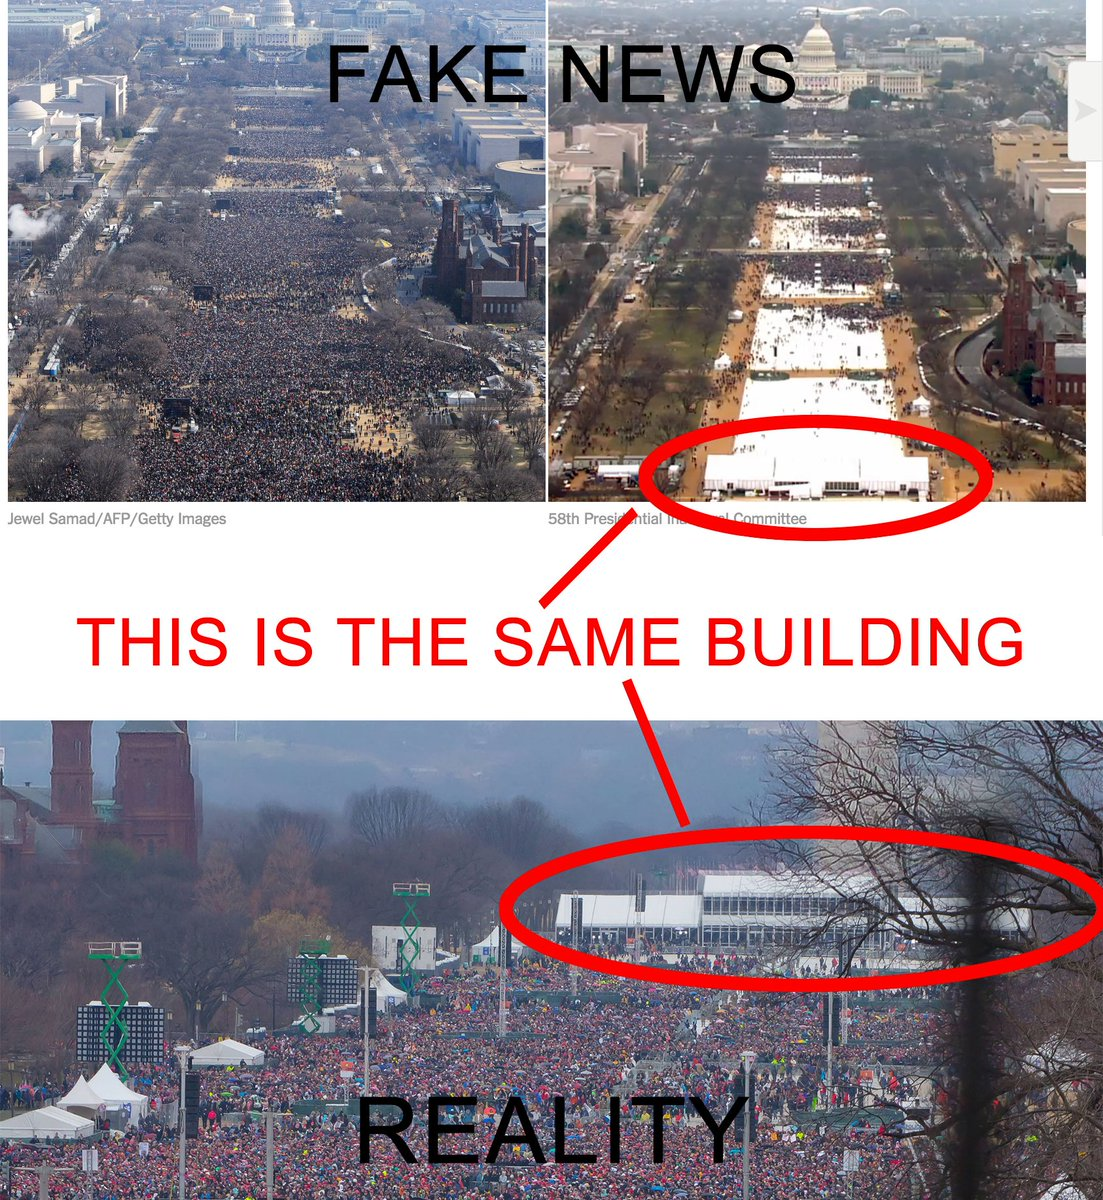
\includegraphics[width=0.5\columnwidth]{trump.jpg}
    \caption{%
      How can someone prove they were there?
      Image: reddit.
    }%
  \end{figure}
\end{frame}

\begin{frame}
  \begin{remark}
    \begin{itemize}
      \item Protection from \acs{MITM} doesn't prevent relaying.
    \end{itemize}
  \end{remark}
\end{frame}

\subsection{Distance-bounding essentials}

\Cref{DBMF,DBTF,DBDH,DBDF} illustrate the four frauds against which \ac{DB} 
should protect.
These frauds are all variants of relay attacks.
Let Alice and Bob be guards, Carol and David wants to enter, but David is not 
authorized to do so.
In the \ac{DBMF} attack (\cref{DBMF}), Alice collaborates with David to pass 
Bob's authentication step.
When Bob gives David the challenge \(C\), he calls Alice to say he got the 
challenge \(C\) from Bob.
Alice asks Carol the same challenge.
Carol honestly responds with the correct response \(R\) and Alice replies \(R\) 
to David.
Now David can tell Bob the correct response \(R\) to enter.

Common \ac{DBMF} attack scenarios are to make someone else pay for something or 
to steal premium cars with passive keyless entry (by relaying the communication 
between the keyfob and the car).

\begin{frame}
  \begin{figure}
    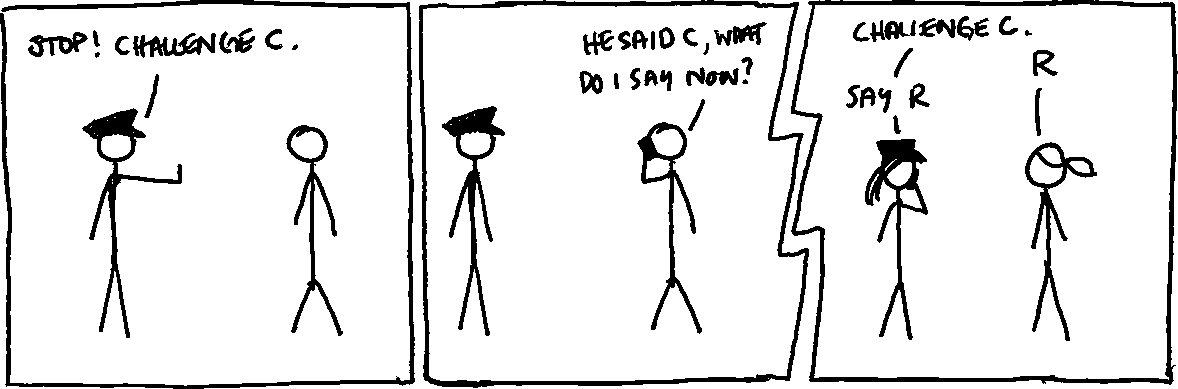
\includegraphics[width=\textwidth]{MF.png}
    \caption{\Acl{DBMF}}\label{DBMF}
  \end{figure}
\end{frame}

\begin{frame}
  \begin{figure}
    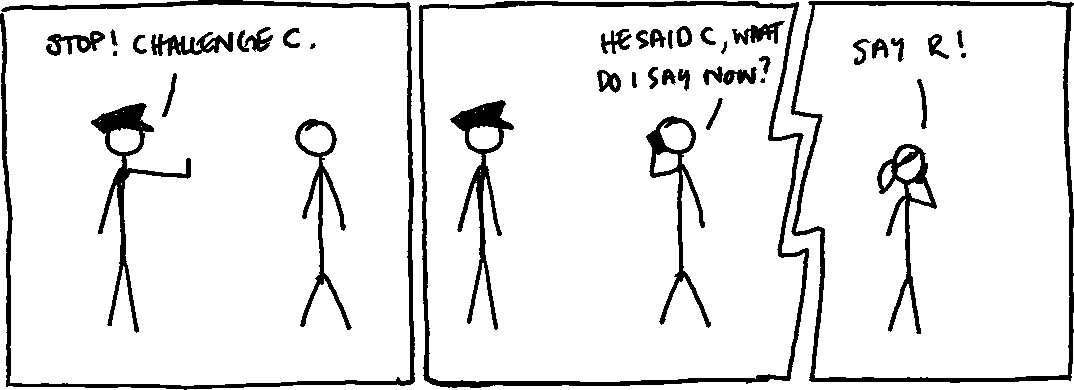
\includegraphics[width=\textwidth]{TF.png}
    \caption{\Acl{DBTF}}\label{DBTF}
  \end{figure}
\end{frame}

\begin{frame}
  \begin{figure}
    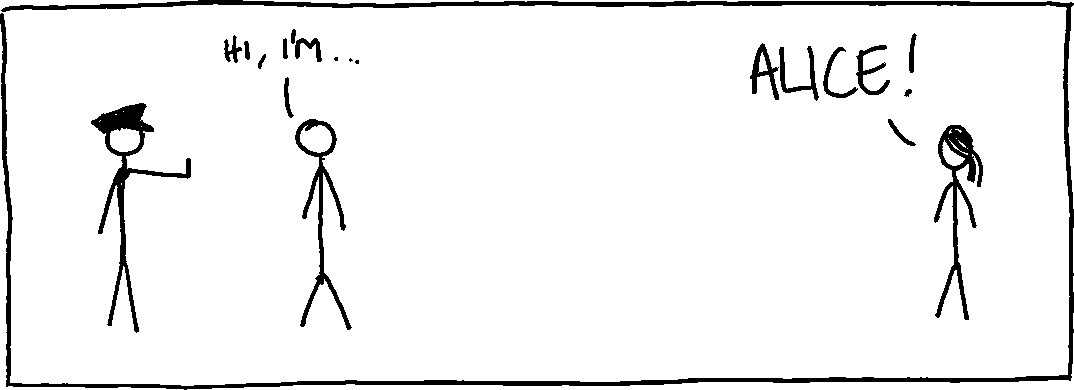
\includegraphics[width=\textwidth]{DH.png}
    \caption{\Acl{DBDH}}\label{DBDH}
  \end{figure}
\end{frame}

\begin{frame}
  \begin{figure}
    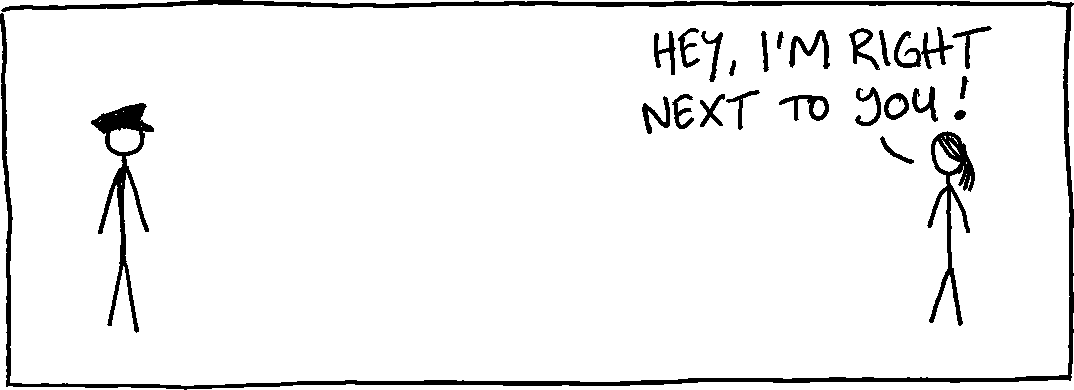
\includegraphics[width=\textwidth]{DF.png}
    \caption{\Acl{DBDF}}\label{DBDF}
  \end{figure}
\end{frame}

The key observation here is that Bob would notice that David calls Alice.
The important part is how we model this detection.
The way Bob will detect that David is talking to Alice, and effectively 
relaying Carol's response to Bob, is by time.
The relay will make David slower to answer the challenge.
If we detect relays by time of flight, we can detect any type of relaying: no 
matter if Bob calls Alice with his phone in plain sight or wears a 
secret-agent-like ear-piece.

Technically, it will be electronics that run the protocol, which means that we 
can do things very fast.
Bob will measure the round-trip time from when he sent the challenge to when he 
received the reply.
If Bob wants to be sure that it is actually David who responds, he can set a 
maximum limit of \eg one metre distance.
Then this round-trip time cannot be longer than the time it would take an 
electro-magnetic wave to travel one metre there and one metre back.
Since electro-magnetic waves travel with the speed of light, the round-trip 
time must be \emph{very small}.

In the \ac{DBTF} attack (\cref{DBTF}), David doesn't need Alice, instead Carol 
collaborates directly with David.
We see that, although we have removed Alice, any form of relay will still be 
detected due to time.
One option for David and Carol is that Carol simply gives her cryptographic key 
to David.
Then David can compute any responses he needs and pass Bob's challenge.
However, we \emph{assume} that Carol wouldn't do that.
Is this a realistic assumption?
If Carol completely trusts David, then it's not.
But there are circumstances when it arguably is.
If this cryptographic key is use to more things than just pass Bob's 
authentication, \eg it is Carol's electronic ID (\eg the Swedish BankID).
Then David could do anything in Carol's name once he has her key, like he could 
transfer all her money to his own account.
If Carol doesn't trust David to not do this, then it is realistic to assume 
that she wouldn't give David a copy of her key.

An example of where this is a realistic attack scenario is public transport.
Where David and Carol can share a single subscription.
However, if the two cannot use the subscription simultaneously, David's 
unlimited use might temporarily lock Carol out.
This inconvenience can serve as the incentive that validates the assumption.

In the \ac{DBDH} attack (\cref{DBDH}), David tries to authenticate to Bob.
But Alice wants to trick Bob into believing that David is Alice (against 
David's will).
By letting David do the bulk of timed responses, Alice might be able to time 
just a few key parts to make Bob believe that he is talking to her instead of 
David.
\Ac{DBDH} is sort of a special case of \ac{DBDF} (\cref{DBDF}), where Alice is 
simply trying to convince Bob that she is close when she actually isn't.

Both of these attacks are realistic when Alice, \eg, must register that she was 
physically present.
For instance, she must prove to her employer that she was at the office.
(For this scenario we find \ac{DBTF} also very relevant, since Alice might 
collaborate with a colleague at the office otherwise.)

\mode<presentation>{%
\begin{frame}
  \begin{question}
    \begin{itemize}
      \item How does a device know that another device is \emph{actually} 
        present?
    \end{itemize}
  \end{question}

  \pause

  \begin{idea}[\Acl*{DB}~\cite{DistanceBounding}]
    \begin{itemize}
      \item Measure round-trip time to estimate maximum distance.
      \item \dots for the authentication.
    \end{itemize}
  \end{idea}
\end{frame}
}

\section[\acs*{DB} \acsp*{ZKPK}]{Distance-bounding \aclp*{ZKPK}}

Now we will turn to the problem of \ac{DB} and the contribution of the paper in 
\cref{db-schnorr-paper}.
Above, we left the problem of how does a witness know that the protester is 
actually present?
\Ac{MITM} protection does not protect from \emph{relaying}, for this we need 
\ac{DB}.

\subsection{Our contribution}

Most protocols in the area of \acl{DB} are symmetric.
This means that the verifier must be trusted.
This doesn't work with the crowd counting scenario above, since by design the 
witnesses must be trusted to keep the protester's \ac{eID} keys secret.
The alternative approach is asymmetric, or public-key based.
However, all are identity-based, but possibly anonymous (as in group or ring 
signatures).
We need Sybil-proof pseudonymity, which none of the existing schemes can 
provide.

\Textcite{SelfCertifiedSybilFreePseudonyms} constructed such self-certified 
Sybil-free pseudonyms from the anonymous-credential scheme by 
\textcite{HowToWinTheCloneWars}.
These are based on \ac{ZKPK} for discrete logarithms.
While \citeauthor{SelfCertifiedSybilFreePseudonyms} worked purely in the 
non-interactive domain, the foundation by \citeauthor{HowToWinTheCloneWars} 
could be both interactive and non-interactive.
The protocol by which they achieve the \ac{ZKPK} property they need is the 
Schnorr identification scheme~\cite{Schnorr}.
This protocol is \iac{ZKPK} for discrete logarithms, but not \acl{DB}.
Our contribution is \iac{DB} version of the Schnorr protocol.
Hence, by replacing the Schnorr protocol by our DB-Schnorr version in any 
protocol where it is used, we make that protocol \acl{DB} --- and hence 
resistant to the relay attacks presented above 
(\cref{illustrations-DB-frauds}).
From the work of 
\textcite{SelfCertifiedSybilFreePseudonyms,HowToWinTheCloneWars} we can then 
construct the \emph{\acl{DB}} Sybil-proof pseudonyms that we need for the crowd 
counting.

\mode<presentation>{%
\begin{frame}
  \begin{solution}
    \begin{itemize}
      \item Adds protection against \acs{DB} attacks to Schnorr~\cite{Schnorr}:
        \begin{itemize}
          \item \Acl{DBDF}
          \item \Acl{DBDH}
          \item \Acl{DBMF}
          \item \Acl{DBTF}
        \end{itemize}

      \item Two versions:
        \begin{enumerate}
          \item Mutual trust
          \item \acs{PKI} based
        \end{enumerate}

      \item Proven in the DFKO model and Tamarin.
    \end{itemize}
  \end{solution}
\end{frame}

\begin{frame}
  \begin{example}[Use cases]
    \begin{itemize}
      \item Distance bounding Direct Anonymous Attestation (TPM standard).
      \item Distance bounding, privacy-preserving attribute-based credentials 
        (CL04 \etc).
    \end{itemize}
  \end{example}
\end{frame}
}

\subsection{Performance}%
\label{performance}

\mode<presentation>{%
  \begin{frame}
    \begin{question}
      \begin{itemize}
        \item How costly is this compared to non-\acs{DB} Schnorr?
      \end{itemize}
    \end{question}
  \end{frame}
}

We will now review the performance of the proposed protocols.
Since the construction is designed as a drop-in replacement for the Schnorr 
identification-scheme~\cite{Schnorr} as \iac{ZKPK} protocol, we will focus on 
how much we must \enquote{pay} for the \ac{DB} property.
We summarize the results in \cref{performance-overview}.

\begin{frame}
  \begin{table}
    \centering
    \caption{%
      A summary of how costly \acl*{DB} is in terms of randomness, arithmetic 
      operations (addition, multiplication), exponentiations and pairing 
      operations.
      \(m, l\in \mathcal{O}(\log \lambda)\) and we must repeat the protocol 
      \(n\) times to achieve desired soundness.
    }\label{performance-overview}
    \begin{tabular}{lrrrr}
      \toprule
      Protocol
      & Rand.~(\si{\bit})
      & Arith.~(\(+, \times\))
      & Exp.
      & Pairings\\
      \midrule
      Schnorr             & \((\lambda+l)n\)  & \(3n\) & \(3n\) & 0\\
      DB, mutual          & \((\lambda+ml)n\) & \(3mn\)& \(3n\) & 0\\
      DB, \acs*{PKI} \(\sum\)
                          & \(4\lambda + (5\lambda + ml)n\)
                          & \((10m+8)n\)
                          & \(9 + 16n\)
                          & \(14\)\\
      ---\acs*{DHKE}      & \(2\lambda\)      & 0    & 4      & 0\\
      ---CL04 blind       & \(2\lambda\)      & 0    & 5      & 8\\
      ---DB               & \(5\lambda + ml\) & \(10m + 2\) & 6 & 0\\
      ---Verification     & 0    & 6 & 10 & 6\\
      \bottomrule
    \end{tabular}
  \end{table}
\end{frame}

\paragraph*{Mutual trust}

We start with the mutual-trust version of the protocol in \cref{DB-Schnorr-UWB} 
(see \cref{DB-Schnorr-UWB-figure}).

In \emph{one round} of the protocol, the cost of the verifier is that of 
generating \(m\) number of \(l\)-bit strings, instead of only one.
This costs the verifier a factor \(m\) of randomness.
The cost of the prover is that of computing \(m\) number of replies (\(s\gets 
\rho - c \alpha \mod q\)), instead of only one.

To achieve security, the protocol must be repeated \(n\) times.
We have the \(l\)-parameter which controls the soundness of the \ac{ZKPK} and 
the \(m\)-parameter controls the soundness of the \acl{DB}.
If we want to achieve 80 bits of security, we can let \(l = m = 6\) (remember, 
\(l\) must be logarithmic in the security parameter) and \(n = 14\).
This makes \acl{DB} a factor \(6\) more expensive over the 
\emph{malicious-verifier secure} Schnorr protocol.

\paragraph*{\acs*{PKI}}

The \ac{PKI} version of the protocol (\cref{DB-Schnorr-PKI,DBSHW-overview}) 
performs one signature verification and four additional proofs in parallel.
The cost for the verifier is one signature verification 
(CL04~\cite{CLsignatures}) in addition to the factor \(m\) of randomness used.
On the prover side, we have the computations for the signature verification and 
four additional proofs in parallel, this changes the cost to a factor of \(5m\) 
for the prover: the prover must compute \(s_i = \rho - c_j \alpha_i\) for 
\(i\in \{1, \dotsc, 5\}, j\in \{1, \dotsc, m\}\).

The cost of the signature is the same as for Anon-Pass~\cite{AnonPass}, which 
implements a public transport pass using this signature scheme.
This signature verification introduces more additions, multiplications, 
exponentiations and pairing operations.
However, the signature will only be blinded and verified once, so this 
represents a constant factor.
It is sufficient to verify it once and reuse the same blinding for all \(n\) 
repetitions of the protocol.
(The same is true for the \ac{DHKE}.)
Thus it is only the \acl{PK} that must be rerun \(n\) times.

\paragraph*{Bit-by-bit}

The traditional bit-by-bit version of the protocol 
(\cref{DB-Schnorr-nbit,DB-Schnorr-nbit-figure}) is not as efficient.
That is due to \(m = 2\) being fixed in this case (there are only two responses 
to choose from), and consequently, we must have a larger value for \(n\) to 
achieve the desired security.




\section{Conclusions}

\mode<presentation>{%
\begin{frame}
  \begin{block}{Contributions}
    \begin{itemize}
      \item Distance-bounding Schnorr protocol
      \item Drop in replacement for Schnorr to add \acl{DB} to any protocol.
      \item \Eg distance-bounding privacy-preserving attribute-based 
        credentials based on \cite{HowToWinTheCloneWars}
    \end{itemize}
  \end{block}
\end{frame}
}

One insight is that we cannot provide deniability in the crowd counting 
scenario.
Deniability is at odds with Sybil resistance.
Since the pseudonym of the protester is a deterministic function of the 
protester's key and the protest's cause identifier, Eve can use that pseudonym 
as a commitment.
She can recompute the pseudonym, see if it is in the set of pseudonyms that 
claimed participation or not.
However, Eve must have access to Alice's key to do this verification.
Due to anonymity, to learn who participated Eve must do this verification for 
the entire population that she is interested in, this is expensive.

Another potential attack to consider is framing:
Eve dislikes the head-of-opposition~Alice, it is not unlikely that she would 
like to frame Alice for participating in a protest to smear Alice.
When Eve verifies if Alice participated in a particular protest, as outlined 
above, she could take the opportunity to try to generate a proof of 
participation.
While the cryptographic aspects of the proof would verify correctly, Eve cannot 
control the time-stamping service.
So any honest verifier would reject it since its time interval would not verify 
correctly.
So even if Eve has access to Alice's key, she cannot forge the temporal 
eligibility\footnote{%
  At the very least, she might not be able to forge a witnessing for spatial 
  eligibility either.
}.

How does this differ with voting?
In voting it is well-established that Alice must be able to deny voting in any 
particular way.
Participation in a vote is also \emph{undeniable}, it is how the vote was cast 
that is deniable.
This works for questions with a few given alternative answers, Alice can deny 
what she answered, but not that she answered.
This is different for petitions or protests, where Alice's mere participation 
implies her opinions.

%\begin{frame}
%  \begin{greenblock}{Possibilities}
%    \begin{itemize}
%      \item We can implement this by extending BankID.
%      \item There are blockchains (ledgers) with reasonable transaction 
%        throughput, \eg OmniLedger.
%    \end{itemize}
%  \end{greenblock}
%
%  \pause
%
%  \begin{alertblock}{Limits}
%    \begin{itemize}
%      \item Cannot trust results that are pro-government if government issues 
%        credentials (Sybil).
%
%      \item Needs transparency and accountability in issuing.
%
%      \item Requires a chip in smartphones for distance bounding.
%    \end{itemize}
%  \end{alertblock}
%\end{frame}

\paragraph*{Future work}

%\mode<presentation>{%
%\begin{frame}
%  \begin{block}{Future work}
%    \begin{itemize}
%      \item Formally prove the protocols.
%      \item How hard to Sybil attack the parliamentary election?
%      \item Turn analog IDs into digital ones?
%    \end{itemize}
%  \end{block}
%\end{frame}
%}

While working on this topic, the following question emerged:
how difficult would it be for a nation state, \eg Sweden, to perform a Sybil 
attack on the identity system?
Certainly, it is easier to cheat in the elections in some states and more 
difficult in others.
But how difficult is it to cheat significantly in an election in a Western 
democracy, such as Sweden?

Now, this type of \enquote{analogue} identity management that are used for 
paper-based elections has been well established for a long time in most parts 
of the world.
Digital identities, however, are not as well established.
There are only certain countries which has a coverage of more than \SI{90}{\%} 
of the population.
How can we turn these \enquote{analogue} identity certificates (\eg passports) 
into digital ones, while preserving privacy and without introducing additional 
trust?
For instance, with the Swedish BankID we convert an analogue ID to a digital 
one, but the way this is done introduces another entity (the banks) that a 
verifier must trust to do the check of the analogue ID correctly.
Can we at least reduce the amount of new trust that we must introduce?
There are suggestions such as proof-of-personhood~\cite{proof-of-personhood} 
that will never scale.

\mode<presentation>{%
  \begin{frame}
    \begin{center}
      Questions, comment, other thoughts?
    \end{center}
  \end{frame}
}
